\documentclass[en]{../../../eplsummary}

\hypertitle{Distributed}{8}{INGI}{2345}
{Nicolas Houtain \and Gorby Nicolas Ndonda Kabasele}
{Peter Van Roy}
$$$$

Attention : This summary is actually based on course note


(Need slide to understand)

\section{Parallel and distributed computing}
\begin{itemize}
    \item Parallel computing : many node, optimize performance, no
        failure
    \item[$\to$] Tightly coupled(low latency/delay and high performance)

    \item Distributed computing : many node in collaboration with
        \textcolor{red}{partial failure}
    \item[$\to$] Loosely coupled(high latency and low perfomance)
\end{itemize}

\section{Consensus}

Atomic broadcast $\equiv$ consensus (proof slide 13)

It's possible to resolve consensus if we have atomic broadcast and vice-versa.
\begin{enumerate}
    \item broadcast $\to$ consensus : We take the first proposal as they have an order 
    \item consensus $\to$ broadcast : The subject of the consensus is the order to take.
\end{enumerate}

Paxos est ce qui est le plus utilisé pour les consensus (TODO)

\section{Modeling distributed system}

\begin{itemize}
    \item Asynchronous : There is no bound on the time for a message to arrive and to be computed, it resolve consensus iff 0 node crashes
    \item Partially synchronous : It start asynchronous and then become
        synchronous(it get an upper bound, we know it will happen but we
        don't know when.)
	  Consensus sit < $\frac{n}{2}$ crashes
    \item Synchronous : Bound known for delivering and computation of message. Consensus with n-1 crashes
\end{itemize}

\paragraph{Asynchronous vs Synchronous}

Bound is simulated with a expect bound to be in partially synchronous.

\section{Failure node}
Bound exist but we don't know the exact value because this bound can
change with time (if RTT increase for example)

We need to adapt the bound.

\begin{itemize}
    \item \textbf{Byzantine faults} : Sending wrong information, omit
        messages,\ldots
        \begin{enumerate}
            \item[$\to$] Byzantine algorithm tolerate $1/3$ faulty node and
                non-byzantine only $1/2$
        \end{enumerate}
    \item \textbf{Self-stabilizing} : It's important to know that system
        can be in a \textit{legitimate} or an
        \textit{illegitimate} state.

        It's robust to failure and don't need initialization!

        \begin{enumerate}
            \item[Need] 
                \begin{enumerate}
                    \item Convergence = from any illegitimate state,
                        system can eventually goes to a legitimate state
                    \item Closure = if in legitimate state, it remains
                        in a legitimate state.
                \end{enumerate}
        \end{enumerate}
\end{itemize}


\section{Formal models of distributed system}

\subsection{Modeling}

\begin{itemize}
    \item Continuous model : described by differential equations
    \item \textbf{Discrete event models} : described by state transition systems
\end{itemize}

Modeling need to be : Complete, Correct and Concise!

\subsubsection{State transition system}
$STS \equiv$ a set of states + rule for transition function
+ set of initial states

\begin{enumerate} 
    \item[$\to$] like finite state machine but no input
\end{enumerate}

\begin{itemize}
    \item A \textbf{configuration} is a snapshot of state of all node

        $$ C =(q_0, q_1, q_2,\cdots, q_{n-1}) $$  where $q_i$ is state of node $p_i$.
\end{itemize}

\paragraph{Property}
Determinism, I/O and atomicity.



\subsubsection{Node}
Can send, receive messages and do local computations.

A state is define by triple $<l, O, s>$ :
\begin{itemize}
    \item $l$ : inbuffer set for each neighbor
    \item $O$ : outbuffer set for each neighbor
    \item $s$ : local state
\end{itemize}

\begin{figure}[h]
    \centering
    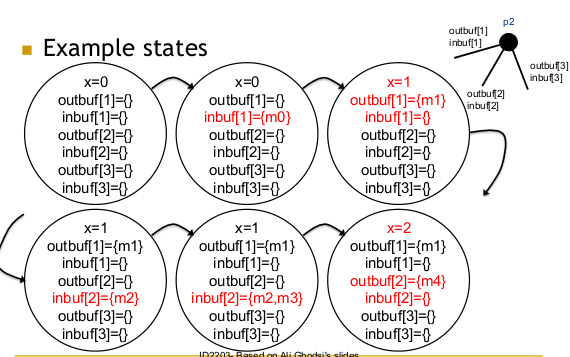
\includegraphics[width=10cm]{img/node.png}
    \caption{Example states}
\end{figure}

\paragraph{Working}
\begin{enumerate}
    \item Waite for message
    \item When receive message, do some computation and send message
    \item Goto 1.
\end{enumerate}

\paragraph{Events}
\begin{itemize}
    \item comp(i) : computation event at process i. 

        \textit{Apply transition function f on node i state}

    \item del(i, j, m) : delivery event of msg m from i to j

        \textit{Move m from outbuf of $p_i$ to inbuf p $p_j$}

\end{itemize}

\subsubsection{Transition functions}
%TODO


\subsubsection{Execution}
An execution is a infinite sequence of ``$config_0, event_1, config_1,
event_2, config_2,\cdots$''


\begin{itemize}
    \item[If] $event_k = comp(i)$ : $config_{k-1}$ change to $config_k$
        by applying $p_i$'s transition function on i's state in
        $config_{k-1}$
    \item[If] $event_k = del(i, j, m)$ : $config_{k-1}$ change to $config_k$
        by moving m from i's outbuf to j's inbuf
\end{itemize}


\subsubsection{Property}

\begin{itemize}
    \item For each comp(i) is associated a \textbf{transition} $(state_1, state_2, i)$
    \item Transition $(s_1, s_2, j)$ is \textbf{applicable} in
        configuration c if  accesible state of node $j$ in c is $s_1$ 
    \item del(i, j, m) \textbf{application} in configuration c if m is
        in outbuf for link i-j of node i in c

    \item \begin{enumerate}
            \item if transition e=($s_1, s_2, i$) is applicable
            \item or if e=del($i, j, m$) is applicable
        \end{enumerate}
        to configuration c, then app(e,c) is the new configuration after
        the event comp(i) or del($i,j,m$)

\end{itemize}


\subsection{Asynchronous (Schedules) / Synchronous}
Non-determinism come from asynchrony(messages take arbitrary time to 
be delivered, and the time to compute varies)\ldots

%TODO


\subsection{Order of event}
The order in which two applicable computation events or
two applicable delivery events are executed is irrelevant!\\
A schedule is a sequence of events. Given the initail configuration, it 
determines the whole execution. Since:
\begin{itemize}
	\item del($i,j,m$) determines the message asynchrony
	\item comp($i$) determines the proccess speed.
\end{itemize}
The non-determinism is embedded in schedule.
\subsection{Admissible execution (Fairness)}
An execution is admissible if:
\begin{itemize}
	\item Each process has infinite number of comp(i).
	\item Every message m sent is eventually del($i,j,m$).
\end{itemize}
The infinity property permit messages to wait arbitrary long times before
being delivered.
\subsection{Synchronus Systems}
The execution is partitionned into disjoints rounds.  A round consist of 
deliver event for all message in outbuf and one compute event on 
every process.

\subsubsection{Causal order $<_H$}
Causal order is \textbf{transitive}.

\begin{itemize}
    \item[$ a <_H b $]
    \item if a occurs befor b on the same process
    \item if a produces m and b delivers m
    \item if a delivers m and b consumes m
\end{itemize}

\paragraph{Concurrent}
a and b are concurrent, $a || b$, if not $a <_H b$ and not $b <_H a$

\subsection{Similarity of execution}
\begin{itemize}
	\item The view of $p_i$ in E, denoted E|$p_i$ is the subsequence 
	of executions E restricted to events and state $p_i$.
	\item 2 executions E,F are similar w.r.r if E|$p_i$ = F|$p_i$.
\end{itemize}
\paragraph{Computation Theorem}
\begin{itemize}
	\item Let E an execution ($c_0,e_1,c_1,e_2,...$) and V the 
	schedule of event ($e_1,e_2,e_3,..$) s.t app$(e_i,e_{i-1})=c_i$
	\item Let P be a permutation of V preserving casual order.
\end{itemize}
Then E is similar to the execution starting in $c_0$ with schedule P. 
\subparagraph{Notations}
similar execution of E,F is noted F~E.
\begin{description}
	\item[Computations or Equivalence class:] A class s.t all the elements
are similar to each other.
\end{description}
Computation theorem implies two importants results:
\begin{enumerate}
	\item There is no algorithm that can observe the order of the sequence
	of events for all executions. %TODO ADD PROOF
	\item Computation theorem does not hold in a model extended s.t each
	process read an hardware clock.%%TODO ADD PROOF
\end{enumerate}
\subsection{Clock}
A clock is used to tell locally if two events are causally related.

\subsubsection{Lamport Clock}
\begin{itemize}
    \item Each process has a local logical clock, t initially t=0.
        Node p piggyback (t, p) on every sent message.
    \item On each event :
    \begin{enumerate}
        \item $t = max(t, t_q) + 1$ : when p receives message with
            timestamp ($t_q, q$) (delivery from q)
        \item $t = t+1$ : for every transistion (comp)
    \end{enumerate}

    \item[$\to$] 
        \begin{itemize}
            \item $(t_p, q) < (t_q, q) IFF (t_p <t_q \vee (t_p = t_q \wedge p <
        q))$
\end{itemize}
\end{itemize}

Lamport logical clock guarantee that if $a <_H b$, then $t(a) < t(b)$

\subsubsection{Vector clock}
\begin{itemize}
    \item Each process has a local vector, $v_p$ of size n. Initially
        $\forall_i v_p[i]=0$

        Node p piggyback $v_p$ on every sent message.
    \item On each event :
    \begin{enumerate}
        \item $v_p[p] = v_p[p] + 1$
        \item $\forall_i : v_p[i] = max(v_p[i], v_q[i])$
    \end{enumerate}

\item[$\to$] \begin{itemize}
        \item $v_p \leq v_q$ iff $\forall_i : v_p[i] \leq v_q[i]$
        \item $v_p < v_q$ iff $v_p \leq v_q$ and $\exists i : v_p[i] <
            v_q[i]$
    \end{itemize}
\end{itemize}

Vector clock guarantee that if $v(a) < v(b)$ then $a <_H b$ but also if
$a <_H b$ then $v(a) < v(b)$

\subparagraph{Precisions}
Vector clock cannot be done with smaller vector than size n for n nodes
\begin{itemize}
	\item The relation $<_H$ is a partial order
	\item The relation < on Lamport is a total order
	\item The relation < on vector is a partial order
\end{itemize}

\subsection{Complexity}
Defined over the 
\begin{itemize}
	\item Number of messages used before terminating
	\item Time it takes to terminate
\end{itemize}
An algorithm has terminated when all states in a config. are terminated
states and there is no more messages in (in/out)bufs.\\
\paragraph{Time Complexity}
A message delay is at most 1 time unit while a computation events take
0 time units. A \textbf{timed execution} is an exectuition s.t
\begin{itemize}
	\item Time is associated with each comp(i) event
	\item First event happens at time 0
	\item Time can never decrease and strictly increases locally.
	\item Max time between comp(i) sending m and comp(j)
	consuming m is 1 time unit.
\end{itemize}
Time complexity is maximum time until termination for all 
admissible timed executions.

\section{Specification and implementation of distributed systems}

\subsection{Event based component model}
There is different model :
\begin{enumerate}
    \item Receive 1 msg and send 1msg
    \item At most receive 1 msg and send at most 1 msg to each neighbor
    \item Receive k msg and send at most 1 msg to each neighbor
\end{enumerate}


\paragraph{ }
Each program consists of a set of \textbf{modules or component
specifications}

\subsubsection{Event}
\begin{itemize}
    \item upon event $<RequestEvent, attr_1, attr_2,\cdots>$ do
            // local computation
            trigger $<ResponseEvent, attr_3, attr_4,\cdots>$
\end{itemize}


There is three man type of event : \textbf{request, indications,
confirmation}


\subsubsection{Modules}

\begin{figure}[h]
    \centering
    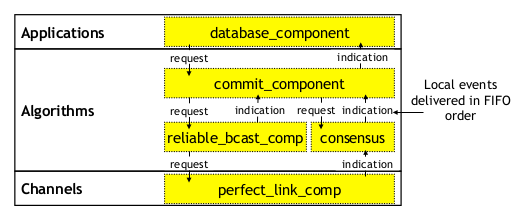
\includegraphics[width=10cm]{img/module.png}
    \caption{Modules scheme}
\end{figure}

\begin{itemize}
    \item receive instruction :  upon event $<delBcaast | src, [data_1,
        data_2,\cdots] >$ do
    \item send instruction :
        trigger $<sendBcast | dest, [data_1, data_2,\cdots]>$
\end{itemize}

\begin{figure}[h]
    \centering
    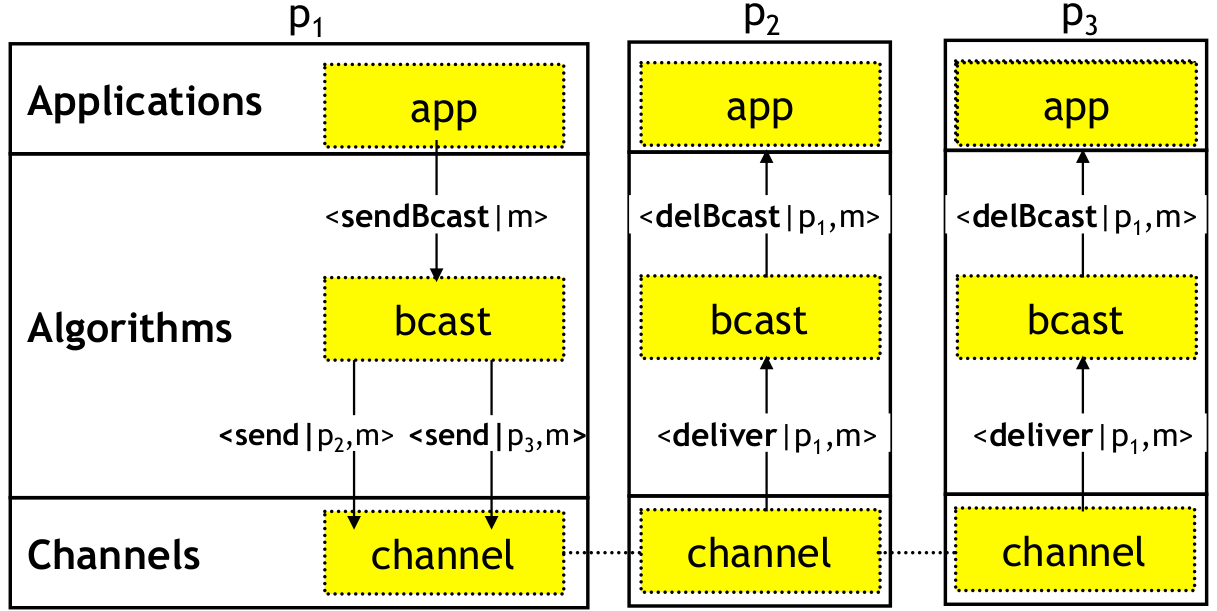
\includegraphics[width=10cm]{img/ex_broadcast.png}
    \caption{Example application uses a broadcast}
\end{figure}


\subsection{Specification of a service}

\begin{figure}[h]
    \begin{tabular}{cc}
        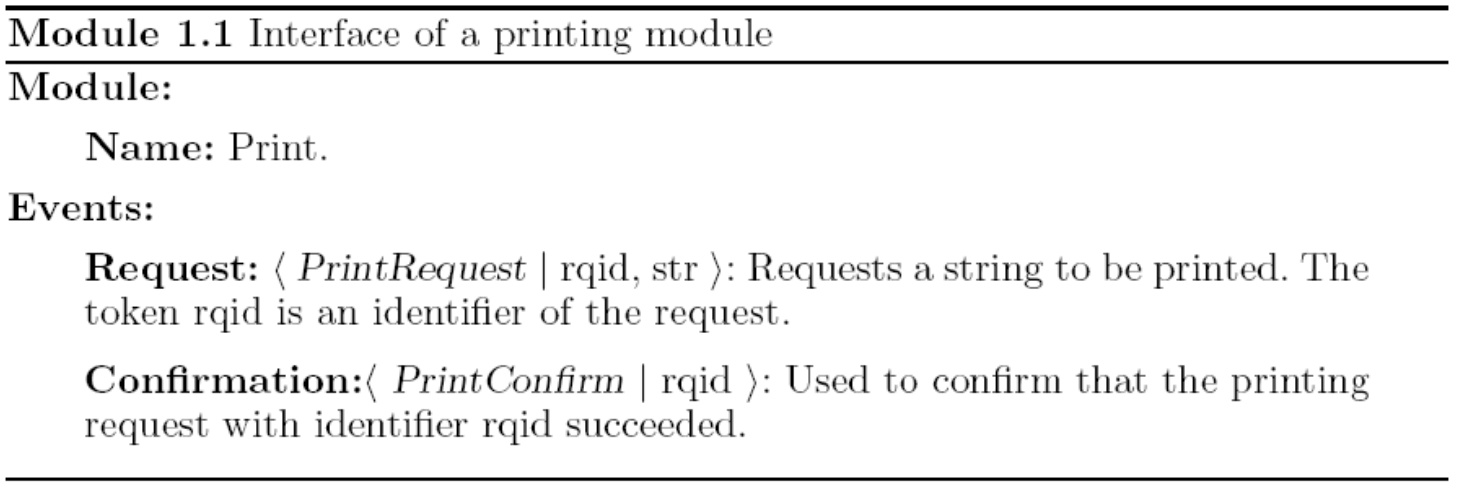
\includegraphics[width=8cm]{img/ex_inter1.png} & 
        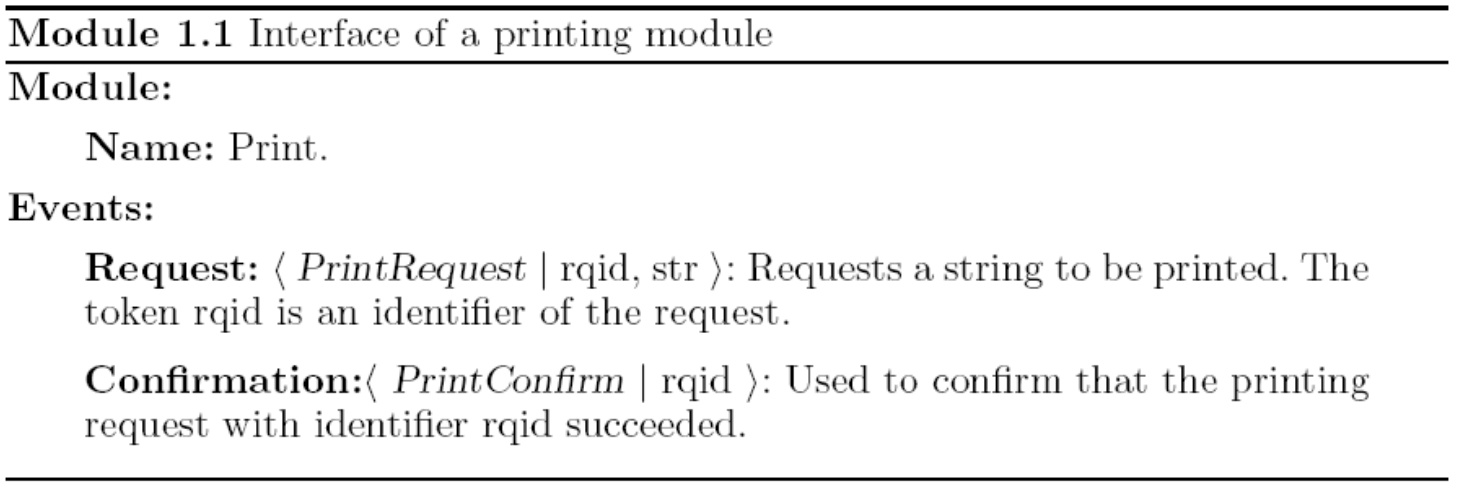
\includegraphics[width=8cm]{img/ex_inter1.png} \\
        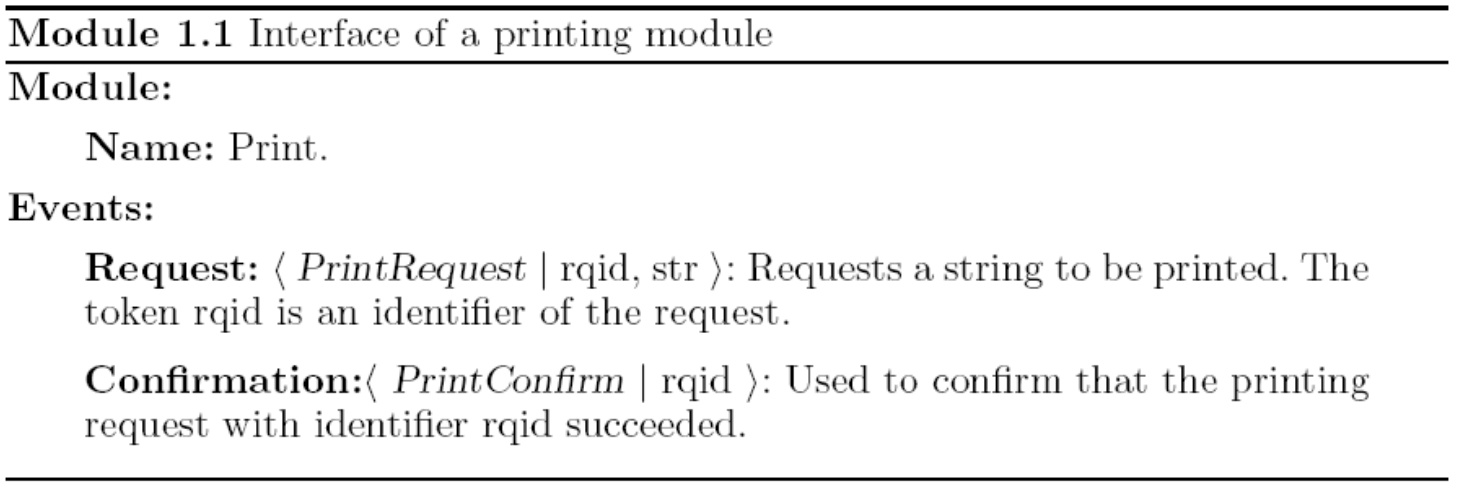
\includegraphics[width=8cm]{img/ex_inter1.png} & 
        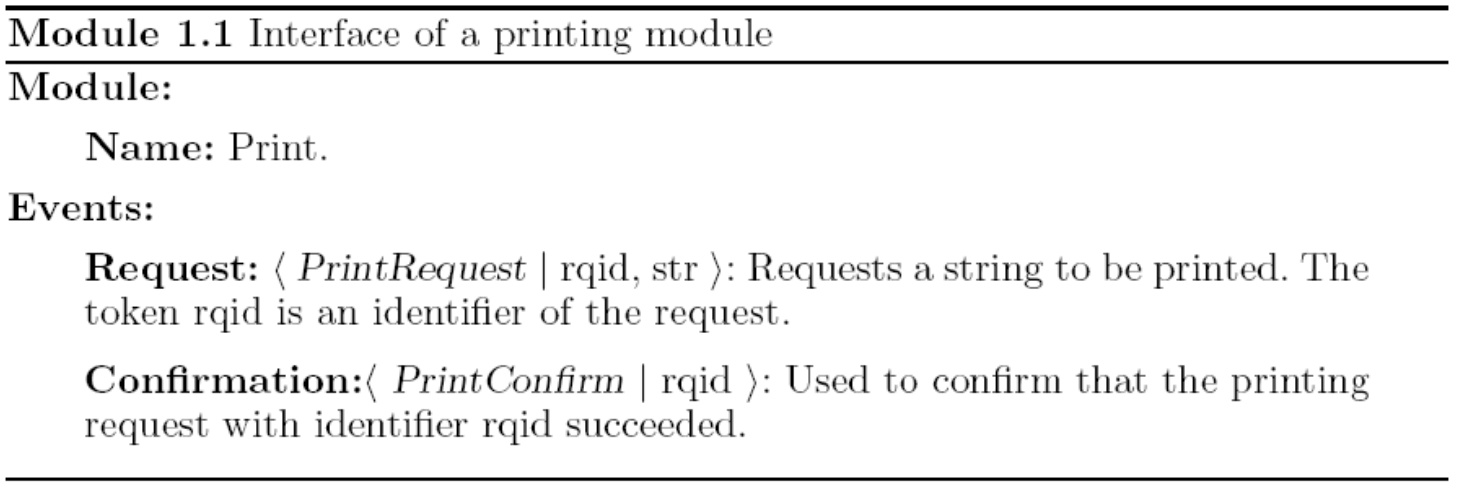
\includegraphics[width=8cm]{img/ex_inter1.png} 
    \end{tabular}
    \caption{Interface example}
\end{figure}


\subsection{Property}

A property P is a function that takes an execution and returns
true/false. (\textit{P is a predicate})

\begin{center}
    \textit{“Any [property] can be expressed as the
conjunction of a safety property and a
liveness property”}
\end{center}

\begin{itemize}
    \item \textbf{Prefix} of a execution E is the first k (for
        some k>0) configurations and events of E
    \item \textbf{Extension} of a prefix P is any execution
        that has P as a prefix

    \item \textbf{Safety} : Properties that state that something bad \textcolor{red}{never}
        happens

        \begin{figure}[!h]
            \centering
            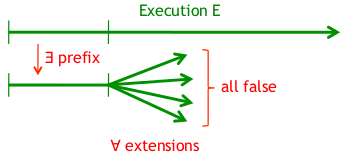
\includegraphics[width=6cm]{img/safety.png}
            \caption{Safety is false if}
        \end{figure}

        \begin{itemize}
            \item[Note:] safety can only be satisfied in infinite time and violated in
                finite time
        \end{itemize}

    \item \textbf{Liveness} : Properties that state that something good
        \textcolor{red}{eventually} happens


        \begin{figure}[!h]
            \centering
            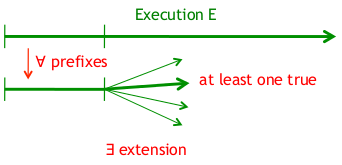
\includegraphics[width=6cm]{img/liveness.png}
            \caption{Liveness is true if}
        \end{figure}


        \begin{itemize}
            \item[Note:] liveness can only be satisfied in finite time and violated in
                infinite time
        \end{itemize}
\end{itemize}


\subsection{Failure}

\subsubsection{Node}

Nodes that don’t fail in an execution are
correct. There is different fail :

\begin{itemize}
    \item \textbf{Crash-stop} : stops taking steps, stops sending/receiving msg

        \begin{itemize}
            \item[$\to$] Cannot recover this failure
        \end{itemize}

    \item \textbf{Omissions} : send (resp. receive) ommission. Formally, an
        event removing element from outbuf[i] (resp. inbuf[i])

    \item \textbf{Crash-recovery} : stops taking steps but receiving and
        sending msg.

        \begin{itemize}
            \item[$\to$] We can recover after crashing with special $<Recovery>$ event
                autmatically generated.

                In practice, restarting in initial recovery state or on
                the save state if we make some (expensive) storage on
                permanent storage device.
        \end{itemize}

        A node is faulty in an execution if it crashes and never
        recovers or crashes/recovers infinitely.

        A correct node may crash and recover.

    \item \textbf{Byzantine} : sending messages/updating its state
        not specified by its algorithm.

        \textit{may behave maliciously, attacking the system}

\end{itemize}

\begin{figure}[h]
    \begin{tabular}{m{8cm}m{7cm}}
        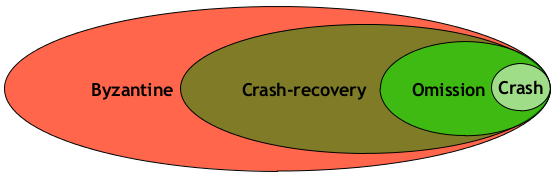
\includegraphics[width=8cm]{img/fault-tolerance.png}
        &
        \begin{itemize}
            \item If node use stable storage : crash-recovery = omission
            \item If node use volatile storage : crash-recovery extend omission
                with amnesia
        \end{itemize}
    \end{tabular}

    \caption{Fault tolerance}
\end{figure}

\subsubsection{Channel}

\begin{itemize}
    \item \textbf{Fair-loss links} : Channel delivers any message sent
        with non-zero probability

        \begin{figure}[h]
            \centering
            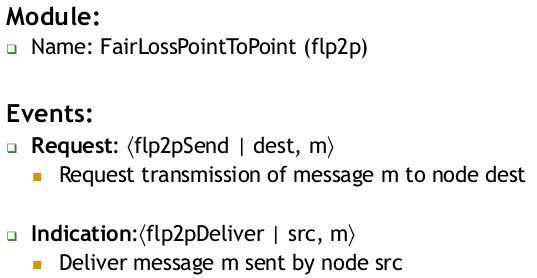
\includegraphics[width=10cm]{img/fairloss.png}
            \caption{Fair-loss links interface}
        \end{figure}

        \begin{enumerate}
            \item FL1. \textbf{Fair-loss} : If m is sent infinitely
                often by $p_i$
                to $p_j$ , and neither crash, then m is delivered infinitely
                often by $p_j$
            \item FL2. \textbf{Finite duplication} : If a m is sent a finite
                number of times by $p_i$ to $p_j$ , then it is delivered a
                finite number of times by $p_j$
            \item FL3. \textbf{No creation} : No message is delivered unless it
                was sent
        \end{enumerate}

    \item \textbf{Stubborn links} : Channel delivers any message sent
        infinitely many times

        \begin{figure}[h]
            \centering
            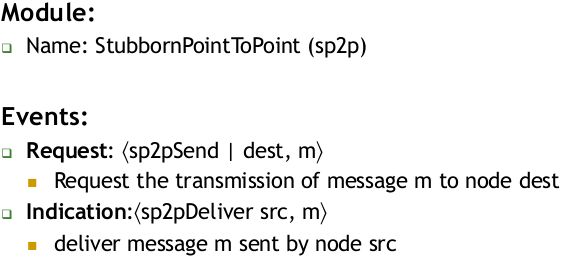
\includegraphics[width=10cm]{img/subborn.png}
            \caption{Stubborn links interface}
        \end{figure}

        \begin{enumerate}
            \item SL1. \textbf{Stubborn delivery} : if a node $p_i$ sends a
                message m to a correct node $p_j$ , and $p_i$ does not
                crash, then $p_j$ delivers m an infinite number of
                times

            \item SL2. \textbf{No creation} : if a message m is delivered by
                some node $p_j$ , then m was previously sent by
                some node $p_i$
        \end{enumerate}

    \item \textbf{Perfect links} : Channel that delivers any message
        sent exactly once

        \begin{figure}[h]
            \centering
            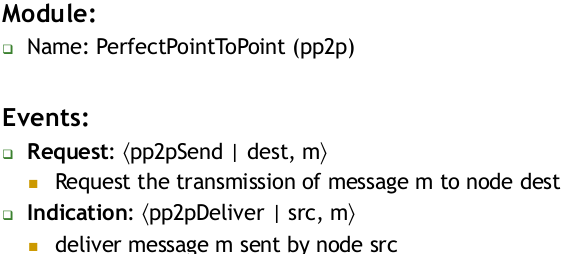
\includegraphics[width=10cm]{img/perfect.png}
            \caption{Perfect links interface}
        \end{figure}

        \begin{enumerate}
            \item PL1. \textbf{Reliable delivery} (liveness) : 
                If neither $p_i$ nor $p_j$ crashes, then every message sent
                by $p_i$ to $p_j$ is eventually delivered by $p_j$

            \item PL2. \textbf{No duplication} (safety) : Every message is delivered
                at most once

            \item PL3. \textbf{No creation} (safety) : No message is delivered unless it was
                sent
        \end{enumerate}

\end{itemize}

\paragraph{Algorithm}


\begin{figure}[h]
    \begin{tabular}{cc}
    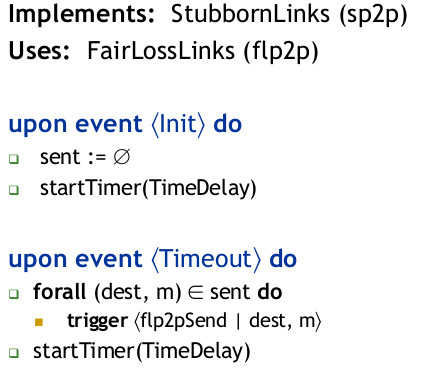
\includegraphics[width=8cm]{img/algo_stubborn.png} &
    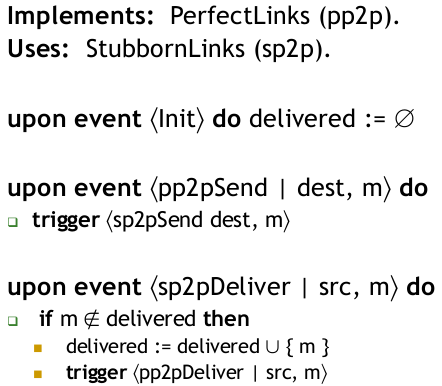
\includegraphics[width=8cm]{img/algo_perfect.png} \\

    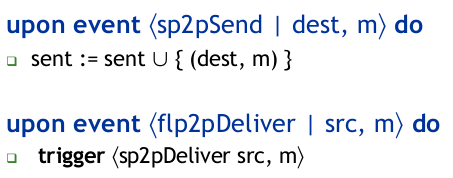
\includegraphics[width=8cm]{img/algo_stubborn2.png}
\end{tabular}
    
    \caption{Implemenation stubborn and perfect}
\end{figure}

\subsection{Timing assumptions}

Different processing speeds of nodes and different speeds of messages.

\subsubsection{Local Vs Global}
\begin{itemize}
    \item Local (one node = State)
        \begin{itemize}
            \item Atomic
            \item Deterministic
        \end{itemize}
    \item Global (many node = Configuration)
        \begin{itemize}
            \item Non-atomic (because piece of code in many node)
            \item Non deterministic (because network and reveiv order message)
        \end{itemize}
\end{itemize}


\subsubsection{Synchronous Vs Asynchronous}
\begin{itemize}
    \item Asynchronous : No timing assumtion on nodes and channels.

        \begin{itemize}
           \item Lamport clocks (or vector clocks) to observe causality. 
           \item Total order not observable
       \end{itemize}

       Internet is asynchronous!

    \item Synchronous : Use round to synchronous (like clock) and this
        is use to detect failure

    \item Partial synchonous : asynchonous system wich eventually
        becomes synchronous.

        \textit{It’s just a way to formalize the following : Your
            algorithm will have a long enough time
            window, where everything behaves nicely
        (synchrony), so that it can achieve its goal}
\end{itemize}


\begin{figure}[h]
    \centering
    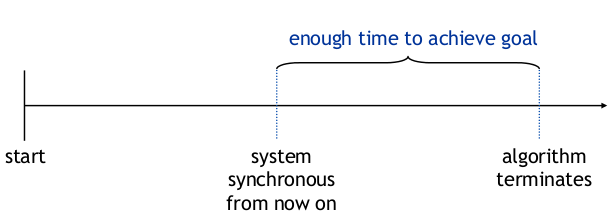
\includegraphics[width=8cm]{img/partialsynchronous.png}
    \caption{Partial synchony}
\end{figure}


\subsection{Failure detectors}

Use failure detectors to encapsulate timing assumtions.
Need completeness and accuracy.

\subsubsection{Typical implementation}
\begin{enumerate}
    \item Periodically exchange \textbf{heartbeat} messages
    \item Timeout based on worst case RTT
    \item if timeout, then suspect node
    \item if rcv msg from suspected node thent revise suspicion and
        increase time-out
\end{enumerate}

\subsubsection{Modeling}

\begin{itemize}
    \item Configuration = state of each node + \textcolor{red}{FD\_state of each
        node}
    \item Transition function on node i gets extra parameter :
        \textcolor{red}{FD\_state of node i}
    \item FD\_state updated in comp(i) by \textcolor{red}{FD\_function}
\end{itemize}

\paragraph{Requirement}
\begin{itemize}
    \item Completeness
    \begin{enumerate}
        \item Strong : Every crashed node is eventually detected by all
            correct nodes

            \textit{here exists a time after which all crashed
            nodes are detected by all correct nodes}

        \item Weak : Every crashed node is eventually detected by some
            correct node

            \textit{There exists a time after which all crashed
            nodes are detected by some correct node}
    \end{enumerate}
    \item Accuracy
        \begin{enumerate}
            \item Strong : No correct node is ever suspected

            \item Weak : There exists a correct node which is never
                suspected by any node

            \item Eventual Strong accuracy : After some finite time the
                FD provides strong accuracy
            \item Eventual Weak accuracy : After some finite time the FD
                provides weak accuracy
        \end{enumerate}
\end{itemize}

\subsubsection{Different established detectors}

\begin{table}
    \begin{tabular}{c|c|c|c|c}
        & & \multicolumn{2}{c}{ Completeness} & \\
        & & Strong & Weak & Order\\
        \hline

        \multirow{2}{*}{Synchm} & Strong accuracy & Perfect detector (P) &
        Detector (Q) & (1) \\
        & Weak accuracy & Strong detector (S) & Weak detector (W) & (2) \\

        \hline

        \multirow{2}{*}{Asyn} & Strong accuracy & Eventually perfect detector
        ($<>P$) & Eventually detector Q ($<>q$) & (3) \\
        & Weak accuracy & Eventually strong detector ($<>S$) & Eventually weak detector
        ($<>W$) & (4) \\
    \end{tabular}
    \caption{$4 \preceq 3, \quad 4 \preceq 2, \quad 2 \preceq 1, \quad 3
    \preceq 1$}
\end{table}

Weak and strong are equivalent. (Weak equivalence $\preceq$ Strong
equivalence is trivial. L'inverse est effectué gràce à un broadcast des
suspect node)


\paragraph{Perfect detector}

\begin{figure}[h]
    \begin{tabular}{cc}
        
\includegraphics[width=8cm]{img/PDF_int.png} &
        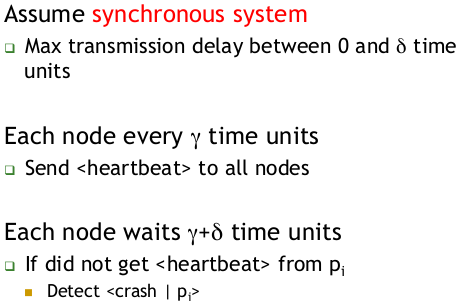
\includegraphics[width=8cm]{img/PDF.png}
    \end{tabular}
        \caption{Implementation perfect detector}
\end{figure}

\paragraph{Eventually perfect detector}
\begin{figure}[h]
    \begin{tabular}{cc}
        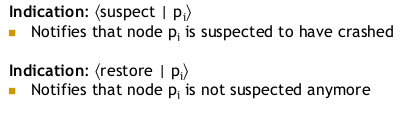
\includegraphics[width=8cm]{img/EPFD_int.png} &
        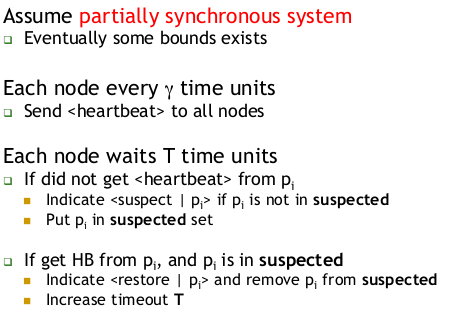
\includegraphics[width=8cm]{img/EPFD.png}
    \end{tabular}
    \caption{Implementation eventually perfect detector}
\end{figure}


\subsection{Leader election}

Note, leader election is a FD : always suspects all nodes except one
(leader).

\paragraph{Which node ?}
Thi lower ID or better the lowest number of crash.

\paragraph{Property}
\begin{itemize}
            \item Completeness : eventually every correct node trusts
            some correct node
            \item Accuracy : No two correct nodes trust different correct nodes
        \end{itemize}

\begin{itemize}
    \item Leader election (LE) which matches P
        \begin{itemize}
            \item Eventual completeness (detects failure)
            \item agreement 
            \item Local accuracy (if a node is elected leader by p i ,
            all previously elected leaders by p i have crashed)
        \end{itemize}
    \item Eventual leader election (LE) which matches $<>$P
        \begin{itemize}
            \item Eventual completeness (detects failure)
            \item Eventual agreement 
        \end{itemize}

\end{itemize}

\subsubsection{Leader election}
\begin{figure}[h]
    \begin{tabular}{cc}
        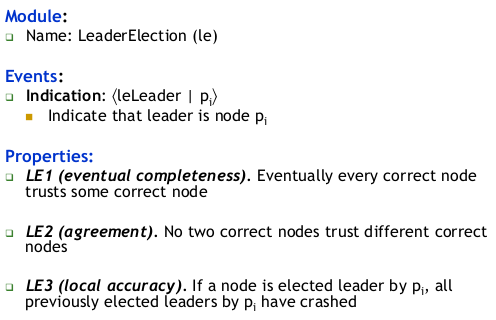
\includegraphics[width=8cm]{img/leader_election_int.png} &
        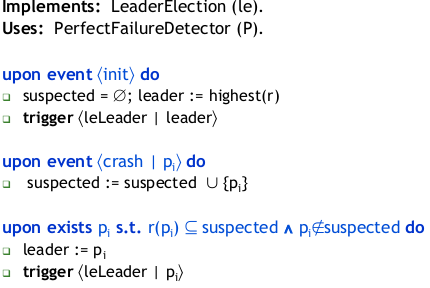
\includegraphics[width=8cm]{img/leader_election.png}
    \end{tabular}
        \caption{Implementation leader election}
\end{figure}

\subsubsection{Eventual leader election}
\begin{figure}[h]
    \begin{tabular}{cc}
        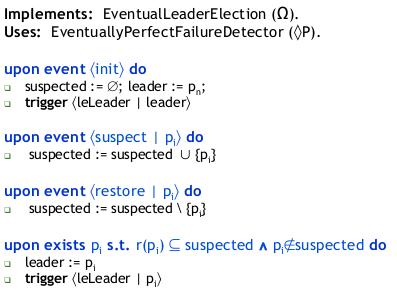
\includegraphics[width=8cm]{img/even_leader_election_int.png} &
        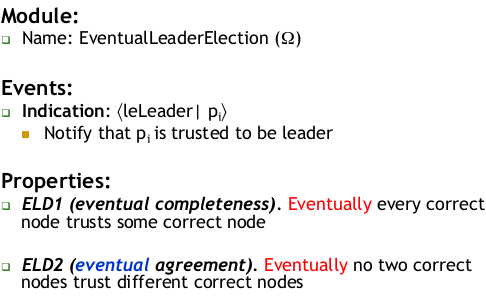
\includegraphics[width=8cm]{img/even_leader_election.png}
    \end{tabular}
        \caption{Implementation eventually leader election}
\end{figure}


\subsection{Reductions}

\paragraph{Preorder $\preceq$} :
\begin{itemize}
    \item Reflexivity
    \item Transitivity
\end{itemize}

\paragraph{Partial order} :
Preorder + antisymmetric


\section{Reliable broadcast}





\begin{thebibliography}{1}
\bibitem{icampus} http://www.icampus.uclouvain.be, {\em Icampus}
\end{thebibliography}

\end{document}
